% Created 2017-12-01 Fri 19:29
% Intended LaTeX compiler: pdflatex
\documentclass[11pt]{article}
\usepackage[utf8]{inputenc}
\usepackage[T1]{fontenc}
\usepackage{graphicx}
\usepackage{grffile}
\usepackage{longtable}
\usepackage{wrapfig}
\usepackage{rotating}
\usepackage[normalem]{ulem}
\usepackage{amsmath}
\usepackage{textcomp}
\usepackage{amssymb}
\usepackage{capt-of}
\usepackage{hyperref}
\usepackage{amsmath}
\author{Jake Brawer}
\date{\today}
\title{Assignment 9}
\hypersetup{
 pdfauthor={Jake Brawer},
 pdftitle={Assignment 9},
 pdfkeywords={},
 pdfsubject={},
 pdfcreator={Emacs 25.3.1 (Org mode 9.1.2)}, 
 pdflang={English}}
\begin{document}

\maketitle


\section*{Problem 1}
\label{sec:org379b3f1}
\subsection*{a)}
\label{sec:org32a3391}
First lets solve for $\mu_{Y}$\\
\begin{align*}
  Y &= \alpha + \beta x + \epsilon\\
  \mu_{Y} &= E\left[Y \right]\\
    &= E\left[ \alpha + \beta x + \epsilon \right]\\
    &= \alpha + \beta \mu_{Y} \tag{1}
\end{align*}

Using $(1)$ we can solve for $\rho$\\
\begin{align*}

  \rho &= \tfrac{cov(X, Y)}{\sigma_{X} \sigma_{X}}\\

       \quad &= E \left[ (Y - \mu_{Y})(X - \mu_{X}) \right]\\

       \quad &= E \left[ (\alpha \beta X + \epsilon - \alpha + \beta \mu_{X} ) (X - \mu_{X})\right]\\

       \quad &= E \left[ \beta (X - \mu_{X})^{2} + \epsilon(X - \mu_{X}) \right]\\

       \quad &= \cfrac{\beta \sigma^{2}_{X}}{\sigma_{X} \sigma_{Y}} \\

  \quad &= \cfrac{\beta \sigma_{X}}{\sigma_{Y}} \tag{2}
\end{align*}

From $(2)$ It's easy to see that $$\beta =\rho \frac{\sigma_{Y}}{\sigma_{X}} $$
and substituting $(2)$ in for $\beta$ in  $(1)$ $$\alpha = \mu_{Y} - \rho
\frac{\sigma_{Y}}{\sigma_{X}} \mu_{X}$$

\subsection*{b)}
\label{sec:org3569c5e}
\begin{align*}

  \sigma_{Y} &= E \left[ (Y - \mu_{Y})^{2} \right]\\

  \quad &= E \left[ (\alpha + \beta X + \epsilon - \alpha - \beta \mu_{x} )^{2} \right] \tag{by Eq. (1)}\\

  \quad &= E \left[ (\beta (X - \mu_{X} ) + \epsilon)^{2} \right]\\

  \quad &= \beta E \left[ (X - \mu_{X})^{2} \right] + E \left[ \epsilon^{2} \right] + E \left[ 2 \beta \epsilon (X - \mu_{X} )\right]\\

  \quad &= \beta^{2} \sigma^{2}_{X} + \mu^{2}_{\epsilon} + 0\\

\end{align*}

So from here we have
\begin{align*}

  \sigma^{2}_{\epsilon} &= \sigma^{2}_{Y} - \beta^{2} \sigma^{2}_{X}\\

  \quad &= \sigma^{2}_{Y} - \rho \cfrac{\sigma^{2}_{Y}}{\sigma^{2}_{X}} \sigma^{2}_{X} \tag{From (a)}\\

  \quad &= (1 - \rho)^{2}\sigma^{2}_{Y}
\end{align*}

\subsection*{c)}
\label{sec:org2699f03}
\begin{align*}
  \tilde{\epsilon} &= \tilde{Y} - \rho \tilde{X}\\
  \quad &= \cfrac{\beta (X - \mu_{X}) + \epsilon}{\sigma_{X}} - \cfrac{\beta \sigma_{X} (X - \mu_{X})}{\sigma_{X}\sigma_{Y}}\\
  \quad &= \cfrac{\epsilon}{\sigma_{Y}}
\end{align*}
Now we can show that $var(\tilde{\epsilon}) = (1 - \rho)^{2}$

\begin{align*}

  \sigma_{\tilde{\epsilon}} &= E \left[ (\tilde{\epsilon} - \mu_{\epsilon})^{2} \right]\\

  \quad &= \tfrac{1}{\sigma_{Y}}  E \left[ (\epsilon - \mu_{\epsilon})^{2} \right]\\

  \quad &= \cfrac{\sigma_{\epsilon}}{\sigma_{Y}}\\

  \text{So we have}\\
  
  \sigma^{2}_{\tilde{\epsilon}} &= \cfrac{\sigma^{2}_{\epsilon}}{\sigma^{2}_{Y}}\\

  \quad &= (1 - \rho)^{2}   \hspace{2in}\text{By problem b) }\\


\end{align*}

\section*{Problem 2}
\label{sec:org9d85282}
\subsection*{a)}
\label{sec:org3e28e9a}
\begin{equation*}
  \left( \cfrac{68 - 65}{3.5} \right) = .85\\

\end{equation*}
So $$1 - \Phi(.85) = 1 - .30 = .70. $$

\subsection*{b)}
\label{sec:orgc51dfb1}
\begin{equation*}
  \left( \cfrac{\hat{Y} - 65}{3.5} \right) = .3 \left( \cfrac{\hat{X} - 70}{4.0} \right)\\
  
\end{equation*}
So
\begin{equation*}
  \hat{Y} = .2625\left( \hat{X} - 70 \right) + 65\\
  
\end{equation*}

\subsection*{c)}
\label{sec:org415b827}
\begin{align*}
  E \left[ y | x = 72 \right]

  &= .2625\left( 72 - 70 \right) + 65\\

  &= 65.525\\

  &= \mu
                               
\end{align*}


\begin{align*}

  \sigma
  &= \sqrt{1 - \rho^{2}} \  \sigma^{2}_{Y}\\

  \quad &= \sqrt{1 -.3^{2}} \  3.5^{2}

  \quad &= 11.1556 
                               
\end{align*}

So $$(Y |X = 72.0) \sim N(65.525, 11.1556)$$

\subsection*{d)}
\label{sec:org4de1921}
$$ \left( \frac{68 - 65.525}{3.34}\right) = .74$$

\section*{Problem 3}
\label{sec:orgeefd5e0}
\begin{verbatim}
library(MASS) # for truehist function
library(rjags)
salary.dat <- read.csv(
  "http://www.stat.yale.edu/~jtc5/238/data/SalariesAndGender.csv"
)
attach(salary.dat)

male <- as.numeric(gender=="m")



m3 <- "
model{
  for(i in 1:12){
    salary[i] ~ dnorm(a + b[1]*male[i] + b[2]*experience[i] + b[3]*male[i]*experience[i], tau)
  }
  a ~ dnorm(0.0, 1.0E-14)
  for(i in 1:3){b[i] ~ dnorm(0.0, 1.0E-14)}
  tau ~ dgamma(.01,.01)
}
"

jmlog <- jags.model(
  textConnection(m3),
  data=list(salary=log(salary), male=male, experience=experience)
)
jm <- jags.model(
  textConnection(m3),
  data=list(salary=salary, male=male, experience=experience)
)

update(jm, 10000)
update(jmlog, 10000)

s <- coda.samples(jm, c("a","b","tau"), 100000)
slog <- coda.samples(jmlog, c("a","b","tau"), 100000)


ss <- as.data.frame(s[[1]])
sslog <- as.data.frame(slog[[1]])

\end{verbatim}


The likelihood that there is a positive interaction in the salary case is:
\begin{verbatim}
mean(ss$'b[3]' > 0)
\end{verbatim}

\begin{verbatim}
0.99058
\end{verbatim}

The likelihood that there is a positive interaction in the log(salary) case is:
\begin{verbatim}
mean(sslog$'b[3]' > 0)
\end{verbatim}

\begin{verbatim}
0.56661
\end{verbatim}

Using the log scale, it is unclear whether the interaction effect is present. Logarithmic scales are nice when you are dealing with data that spans orders of magnitude. In terms of salaries, such vasts differences in salaries are not likely to exists between employees, and so the using a log scale is thus not very useful.

\section*{Problem 4}
\label{sec:orge7c39ab}

\subsection*{a)}
\label{sec:orgddff993}
\begin{verbatim}
source("http://www.stat.yale.edu/~jtc5/238/data/martian-basketball-data.r")
m1 <- "
  model{
    for(i in 1:100){
      ks[i] ~ dbinom( th1[i], ns[i])
      th1[i] ~ dunif(0,1)
    }
}
"

m2 <- "
  model{
    for(i in 1:100){
      ks[i] ~ dbinom(th2[i], ns[i])
      th2[i] ~ dbeta(a, b)
    }
    p ~ dunif(0, 1)
    lam ~ dexp(0.0001)
    a <- lam * p
    b <- (1 - p) * lam
}
"
jm1 <- jags.model (file = textConnection ( m1 ),
                  data=list(ks=ks, ns=ns),
                  )
cs1 <- coda.samples (jm1 , c("th1"), 10000)
s1 <- as.data.frame (cs1 [[1]])

jm2 <- jags.model (file = textConnection ( m2 ),
                  data=list(ks=ks, ns=ns),
                  )
cs2 <- coda.samples (jm2 , c("th2", "p", "lam"), 10000)
s2 <- as.data.frame (cs2 [[1]])

par(mfrow = c(2,2))
truehist(s1$"th1[3]")
truehist(s2$"th2[3]")
truehist(s2$"lam")
truehist(s2$"p")
\end{verbatim}

\begin{center}
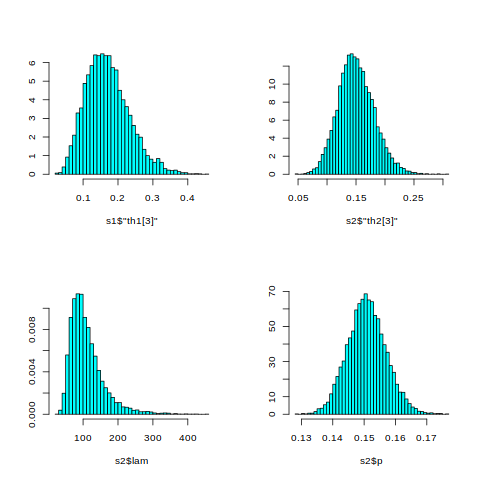
\includegraphics[width=.9\linewidth]{fig1.png}
\end{center}

\subsection*{b)}
\label{sec:org5bd09a6}
\begin{verbatim}
postmeans1 <-  colMeans(s1)
postmeans2 <-  colMeans(s2[, 3:102])

plot(postmeans1,postmeans2)
\end{verbatim}

\begin{center}
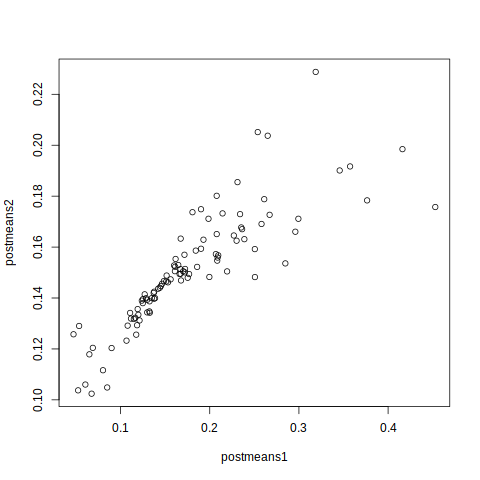
\includegraphics[width=.9\linewidth]{fig2.png}
\end{center}

\subsection*{c)}
\label{sec:org0b31125}

\begin{verbatim}
length(postmeans2)
xlim <- c(0,.5)
ylim <- c(0,.5)
par(mfrow = c(2,1))
plot(postmeans1, trueprobs, col = 1, lim = xlim, ylim = ylim)
abline(coef=c(0,1))
plot(postmeans2, trueprobs, col=1, xlim = xlim, ylim = ylim)
abline(coef=c(0,1))

\end{verbatim}

\begin{center}
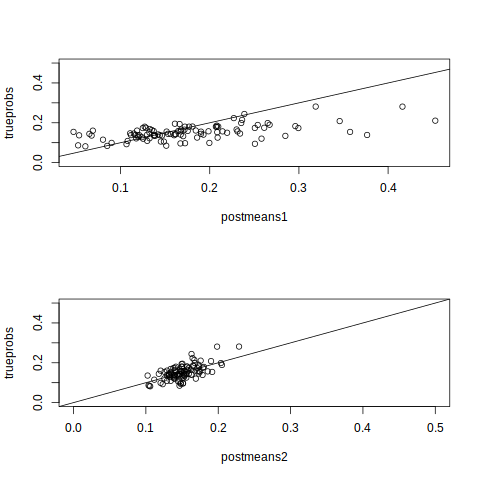
\includegraphics[width=.9\linewidth]{fig3.png}
\end{center}

\subsection*{d)}
\label{sec:org8d63748}

\begin{verbatim}
quant <- c(0.025, 0.975)
M1L <- lapply(s1, quantile, 0.025)
M2L <- lapply(s2[3:102], quantile, 0.025)
M1U <- lapply(s1, quantile, 0.975)
M2U <- lapply(s2[3:102], quantile, 0.975)

M1L[[1]] < M1U[[1]]
nms <- c("trueprobs", "M1L", "M1U", "cover1", "M2L", "M2U", "cover2")
df <- data.frame(matrix(ncol=length(nms), nrow = 100))
colnames(df) <- nms
for(i in 1:100){
  c1 <-  trueprobs[i] >= M1L[[i]] & trueprobs[i] <= M1U[[i]]
  c2 <-  trueprobs[i] >= M2L[[i]] & trueprobs[i] <= M2U[[i]]
  r <- list(trueprobs[i],M1L[[i]], M1U[[i]], c1[[1]], M2L[[i]], M2U[[i]], c2[[1]] )
  df[i,] <- r
}
head(df)
tail(df)
\end{verbatim}

\begin{verbatim}
  trueprobs        M1L       M1U cover1        M2L       M2U cover2
1 0.1341175 0.09808346 0.1869452   TRUE 0.10374789 0.1806429   TRUE
2 0.1732624 0.04940630 0.2321773   TRUE 0.08373924 0.1974685   TRUE
3 0.1326052 0.06724363 0.3122853   TRUE 0.09346874 0.2179882   TRUE
4 0.1443848 0.01385996 0.1535057   TRUE 0.06411825 0.1749340   TRUE
5 0.1585323 0.08861564 0.2551024   TRUE 0.10135107 0.2103108   TRUE
6 0.1808951 0.07434845 0.3932984   TRUE 0.09771855 0.2323512   TRUE
     trueprobs        M1L       M1U cover1        M2L       M2U cover2
95  0.15666284 0.12647688 0.3153460   TRUE 0.12019647 0.2376223   TRUE
96  0.21049344 0.19377363 0.7359731   TRUE 0.10960895 0.2644518   TRUE
97  0.19851406 0.18027855 0.3578279   TRUE 0.14806369 0.2724698   TRUE
98  0.14461626 0.04449855 0.3134686   TRUE 0.08547946 0.2139191   TRUE
99  0.17478313 0.14492910 0.4076666   TRUE 0.12030734 0.2578638   TRUE
100 0.09875627 0.02843607 0.4858974   TRUE 0.08558720 0.2292309   TRUE
\end{verbatim}

\subsection*{e)}
\label{sec:org3d49af7}

\begin{verbatim}
length(df$cover1[df$cover1==TRUE]) /100
\end{verbatim}

\begin{verbatim}
0.95
\end{verbatim}


\begin{verbatim}
length(df$cover2[df$cover2==TRUE]) /100
\end{verbatim}

\begin{verbatim}
0.95
\end{verbatim}

the predicted value is within the interval \$95\$\% of the time for both models, so its hard to judge on those terms alone. Lets look at the average size of each interval

\begin{verbatim}
mu1 <- mean(df$M1U - df$M1L)
sd1 <- sd(df$M1U - df$M1L)
sprintf("Mean interval length for M1: %s, SD: %s", mu1, sd1)
\end{verbatim}

\begin{verbatim}
Mean interval length for M1: 0.222794270035701, SD: 0.123643398032502
\end{verbatim}

\begin{verbatim}
mu2 <- mean(df$M2U - df$M2L)
sd2 <- sd(df$M2U - df$M2L)
sprintf("Mean interval length for M2: %s, SD: %s", mu2, sd2)
\end{verbatim}

\begin{verbatim}
Mean interval length for M2: 0.113894949022019, SD: 0.023634332314039
\end{verbatim}

Clearly model the set of intervals from Model 2 are preferred. While M2 is no more accurate than M1, the intervals more precisely hone in on the predicted value.
\subsection*{f)}
\label{sec:org172972d}
First we will store the best players for each model.
\begin{verbatim}
I1 <- rep(0, dim(s1)[1])
I2 <- rep(0, dim(s1)[1])
ths2 <- subset(s2,select = -c(1,2))
# Save the best player at each iteration for each model.
for(i in 1:dim(s1)[1]){
  I1[i] <- which(s1[i, ] == max(s1[i, ]))
  I2[i] <- which(ths2[i, ] == max(ths2[i, ]))
}
\end{verbatim}

The probability that 19 is the best player according to model 1 is
\begin{verbatim}
length(I1[I1== 19])/length(I1)
\end{verbatim}

\begin{verbatim}
0.0029
\end{verbatim}


The probability that 19 is the best player according to model 2 is
\begin{verbatim}
length(I2[I2== 19])/length(I2)
\end{verbatim}

\begin{verbatim}
0.2631
\end{verbatim}

Clearly Model 2 is the better model.
\end{document}